%# -*- coding: utf-8-unix -*-
%%==================================================
%% chapter03.tex
%%==================================================

%\bibliographystyle{sjtu2}%[此处用于每章都生产参考文献]
\chapter{需求分析}
\label{chap:requirement}
本系统分为3个共享数据库的互相关联又相对独立的模块,需求分析的工作不是仅仅做三遍就行,而是要考虑到相互联系和共用资源。由于整体上是传感器管理系统,所以传感器(Sensor)这个资源肯定是共享的,不同的系统都得有登录和权限管理,所以用户(User)也需要共享,这两种资源需要统一在版本管理系统中管理,这样能够保证所有用户和设备资源的一致性,又能在此基础上各自独立地实现业务逻辑。不同系统上的用户可能实际含义不太相同,本系统使用用户的角色(role)属性来区分,具体角色有:
\begin{description}
  \item[普通用户(user)] Smart Home模块和Smart City模块的最终用户,一个传感器会属于一个普通用户,一个普通用户可以拥有多个传感器。
  \item[管理员(admin)] 版本管理模块的最终用户,也就是Clarity的硬件开发人员和管理人员,除了管理传感器版本等信息外还可以管理用户。
  \item[根用户(root)] 超级用户,给系统维护人员或开发人员的角色,拥有最高权限,可以修改任何资源。
\end{description}

注1:本系统中版本管理模块取名“balanar”,Smart Home取名“robotic”,Smart City名字叫“azwraith”。这3个名字都只做内部代号,但也许会在一些代码或截图中出现,为免误解,特此声明。其中只有robotic(意为机器人的)跟项目内容有点联系,其余两个无实际含义。

注2:本章节中的原型和设计稿都不一定与最终的需求吻合,因为可能有些需求修改没有必要在原型和设计稿上体现。

下面本章将详细从不同的角度对各模块进行需求分析:
\section{版本管理模块}
版本管理模块面向的用户是Clarity的硬件开发人员,原本用户使用Excel记录传感器版本、批次、拥有者等信息。但随着传感器的不断改进和零件的不断进货,有越来越多的版本、批次、兼容性、合作方和制作给合作方的特殊版本,使用Excel的时间成本和精力成本越来越高。版本管理模块的最终用户有三种,都是本系统的管理员,分别是软件开发人员、硬件开发人员和公司管理人员。系统需要能够让用户能够处理传感器、用户、兼容性、硬件版本、固件版本、软件版本、五种零件版本和五种零件批次的增删改查以及这些资源之间的复杂关系,还需要处理一些特殊的格式校验,让用户输入的时候得到及时的校验和反馈。

\subsection{用户用例}
本课题使用Power Designer绘制了一个用例图,如图\ref{fig:balanar_usecase}所示,版本管理模块有如下用户用例:
\begin{enumerate}
  \item 所有用户登录;
  \item 硬件开发者增删改查传感器、硬件版本、固件版本、零件版本、零件批次;
  \item 软件开发者增删改查软件版本;
  \item 硬件和软件开发者增删改查版本兼容性;
  \item 公司管理人员增删改查用户;
\end{enumerate}
\begin{figure}[!htp]
 \centering
 \includegraphics[width=0.8\textwidth]{balanar_usecase.png}
 \bicaption[fig:balanar_usecase]{版本管理模块用例}{版本管理模块用例}{Fig}{Usecase of Version Management}
\end{figure}
\subsection{用户故事}
经过与需求方的多次需求会议,本课题总结出如下主要的用户故事:
\begin{enumerate}
  \item 每当硬件开发人员设计出新版本的零件,需要到系统中添加一个零件版本,填写一些参数,其中ID参数需要严格的格式校验。
  \item 每当硬件开发人员下单订购或者收到一批零件,需要到系统中添加一个零件批次或者修改到货日期,选择相应的一种零件版本。
  \item 每当硬件开发人员准备装配一种拥有新版本零件的传感器,需要到系统中添加一个硬件版本,选择相应的五种零件版本。
  \item 每当硬件开发人员准备装配一种拥有新固件的传感器,需要到系统中添加一个固件版本,并添加对应的兼容性。
  \item 每当硬件开发人员装配完成一批新的传感器,需要到系统中添加这些传感器,选择相应的硬件版本、固件版本和五个零件批次,同时可以指定一个拥有者(普通用户)。
  \item 每当Clarity有新的合作伙伴,Clarity的管理人员可以添加普通用户(角色),将来有给他们专用的传感器时,可以指定为拥有者。
\end{enumerate}
\begin{figure}[H]
 \centering
 \includegraphics[width=\textwidth]{data_model.png}
 \bicaption[fig:balanar_data_model]{版本管理模块 数据模型}{版本管理模块 数据模型}{Fig}{Version Management module's data model}
\end{figure}
\subsection{数据模型}
本课题使用ARIS业务流程建模软件建立了一个数据模型,如图\ref{fig:balanar_data_model}所示,传感器与硬件版本和固件版本有关,同时与五种零件的批次有光,硬件版本由五种零件版本组成,每个零件版本对于很多零件批次,固件版本和硬件版本有兼容性,固件版本和软件版本有兼容性,每个传感器可以属于一个用户,其中灰色的Sales是不在本模块也不在本系统中的:
\subsection{数据库设计:数据字典}
由于本课题使用的MongoDB不是传统的关系型数据库,数据库表设计不是很有必要,所以直接使用普通文本定义了一套数据字典,以免开发过程中混淆不同的资源名和属性名,同时对字段类型做了一些限定,这里只展示了关于传感器资源的定义,详情请看附录A(数据字典)。
\begin{lstlisting}[language={JSON}, caption={版本管理模块的数据字典}]
Sensor: {
  @pk id
  @fk hardwareVersion
  @fk firmwareVersion,
  @fk componentBatches: {body, pcb, photodiode, laser, fan},

  threshold: type(integer),
  noiseLevel,
  calibrations: {
    mass: type(decimal),
    number: type(decimal)
  },
  applicationType: type(enum(SMART_CITY)),
}
\end{lstlisting}

\subsection{快速原型}
本系统在正式开发之前还使用一款叫做balsamiq模拟软件做了一个快速原型,用于和需求方确认基本的界面和操作流程。如图\ref{fig:balanar_mockup}所示,这里只展示了一个页面,详情请看附件快速原型。
\begin{figure}[H]
 \centering
 \includegraphics[width=\textwidth,page=8]{pdf/balanar_prototype.pdf}
 \bicaption[fig:balanar_mockup]{版本管理模块原型样例}{版本管理模块原型样例}{Fig}{Example mockup of Version Management}
\end{figure}

\section{Smart Home模块}
本模块的当前的主要目标客户是一家日本的家电制造企业,最终用户是该企业家电产品的用户。该企业生产的产品是空调和空气净化器等家用电器,因此Clarity为其量身打造了智能家居(Smart Home)解决方案。
\subsection{智能家居解决方案}
首先,目标用户是购买了该企业各种家电和空气净化器的个人或家庭,用户还可以随身携带一个Clarity的个人空气质量传感器。普通的空气净化器只能一直开着或者在人的操控下间歇性地净化空气,而搭载空气质量传感器的家电也只能检测空气质量并报告给用户,并不能实际改善空气质量,Clarity在两者之间引入了一个烧录了智能程序的可编程扫地机器人巧妙地弥补了两者的不足。

如图\ref{fig:robotic_progress}泳道流程图所示,此智能家居解决方案按以下流程工作:
\begin{enumerate}
  \item 不同房间的空气质量传感器持续上传数据到服务器,服务器保存数据;
  \item 服务器定时地计算并评估空气质量的好坏;
  \item 一旦有房间空气质量低于一定水平,服务器就会给机器人下达净化指令,机器人会移动到对应的房间并开启其上搭载空气净化器;
  \item 空气质量好转之后,服务器再给机器人下达停止指令,机器人会关掉空气净化器原地待命;
  \item 用户可以切换手动模式和自动模式,手动模式下服务器自动指令无效,用户可以指定机器人去某个传感器所在的房间,自动模式下用户控制无效;
\end{enumerate}

\begin{figure}[!htp]
 \centering
 \includegraphics[width=\textwidth]{figure/robotic_progress.pdf}
 \bicaption[fig:robotic_progress]{Smart Home模块泳道流程图}{Smart Home模块泳道流程图}{Fig}{BPMN of Smart Home}
\end{figure}

\subsection{用户用例}
本课题使用Power Designer绘制了一张用例图,如图\ref{fig:robotic_usecase}所示,用户有如下用例:
\begin{itemize}
  \item 登录
  \item 查看空气质量指数(AQI)和健康指数(Health Index)
  \subitem 查看个人AQI和健康指数
  \subitem 查看城市AQI和健康指数
  \subitem 查看家里平均AQI和健康指数
  \subitem 查看家里
  \subsubitem 查看房间空气污染情况
  \subsubitem 查看房间历史AQI折线图
  \item 控制机器人
  \subitem 切换机器人到手动模式或自动模式
  \subitem 控制机器人去某个房间,这一点在界面上依赖查看房间空气质量情况
\end{itemize}
\begin{figure}[!htp]
 \centering
 \includegraphics[width=\textwidth]{robotic_usecase.png}
 \bicaption[fig:robotic_usecase]{Smart Home模块用例图}{Smart Home模块用例图}{Fig}{Usecase of Smart Home}
\end{figure}

\subsection{用户故事}
\begin{enumerate}
  \item 用户随时查看个人、家里和城市的空气质量情况和健康指数;
  \item 用户随时家里不同房间的空气质量状况和历史空气质量折线图;
  \item 用户随时查看机器人的位置和空气净化器的工作状态;
  \item 用户随时把机器人切换到手动模式,并控制机器人去任何房间并自动开始净化空气;
\end{enumerate}
\subsection{设计稿}
本模块的需求方给出了一个比较独特且详细的设计稿,如图\ref{fig:robotic_design}所示,这是一个像手风琴一样的页面,个人、家庭、城市三个叶子可以被分别点击展开,这里只展示了一个页面,详情请看附件设计稿。
\begin{figure}[H]
 \centering
 \includegraphics[height=0.8\linewidth, page=2, angle=-90]{pdf/robotic_design.pdf}
 \bicaption[fig:robotic_design]{Smart Home模块设计稿样例}{Smart Home模块设计稿样例}{Fig}{Example design of Smart Home}
\end{figure}

\section{Smart City模块}
本模块的当前主要目标客户是美国一家城市政府,最终用户是政府工作人员。该城市计划大量安装Clarity的传感器以监控城市空气质量,这就需要在智慧城市级别提供空气质量的数据查看和设备管理服务。
\subsection{用户用例}
本课题使用Power Designer绘制了一张用例图,如图\ref{fig:azwraith_usecase},用户具有如下用例:
\begin{enumerate}
  \item 管理设备;
  \subitem 添加设备;
  \subitem 删除设备;
  \subitem 显示设备;
  \subitem 隐藏设备;
  \item 查看数据;
  \subitem 以地图形式查看传感器位置和当前AQI;
  \subitem 以图表形式查看多个设备的最近的AQI,包括实时数据和最新的历史数据;
  \subsubitem 选择时间精度;
  \subsubitem 选择AQI度量;
  \item 保存数据为折线图,此用例依赖以图表形式查看数据的用例;
  \item 导出数据到CSV;
  \subitem 导出最近的AQI数据,此用例依赖以图表形式查看数据的用例;
  \subitem 导出非最近的AQI数据
\end{enumerate}
\begin{figure}[!htp]
 \centering
 \includegraphics[width=\textwidth]{azwraith_usecase.png}
 \bicaption[fig:azwraith_usecase]{Smart City模块用例图}{Smart City模块用例图}{Fig}{Usecase of Smart City}
\end{figure}

\subsection{用户故事}
\begin{enumerate}
  \item 市政部门安装了新的传感器或者拆除了旧的传感器,用户可以在设备列表中添加或删除设备。
  \item 用户想要查看实时数据或者最近的历史数据,可以在图表中查看,可以在图表中调节时间精度和AQI度量。
  \item 用户想要查看设备的具体位置和当前AQI,可以在地图中查看。
  \item 用户想要在图表或地图中隐藏或显示一些设备,可以在设备列表中勾选或取消勾选。
  \item 用户想要保存当前图表为图片,可以在图表的工具栏中点击保存图片。
  \item 用户想要导出当前图表上的数据,可以在图表的工具栏中点击导出CSV。
  \item 用户想要指定时间段下载,可以在图表的工具栏中点击高级下载跳转到或者直接通过地址进入一个单独的下载页面,在表单中选择设备、时间跨度、时间精度和度量,然后点击下载。
\end{enumerate}

\subsection{快速原型}
本系统在开发之初做了一个简单的快速原型,如图\ref{fig:azwraith_mockups}所示。
\begin{figure}[H]
 \centering
 \includegraphics[width=0.7\textwidth]{pdf/azwraith_prototype.pdf}

 \vspace{0.1cm}

 \includegraphics[width=0.7\textwidth, page=2]{pdf/azwraith_prototype.pdf}
 \bicaption[fig:azwraith_mockups]{Smart City模块原型}{Smart City模块原型}{Fig}{Smart City module’s mockups}
\end{figure}

\subsection{设计稿}
但后来因为这个模块比较重要,而且不像版本管理模块不是非常注重UI,公司又请专门的设计师给出了一个设计稿,如图\ref{fig:azwraith_design}所示。
\begin{figure}[htb]
 \centering
 \includegraphics[width=0.75\linewidth]{azwraith_login.jpg}

 \vspace{0.1cm}

 \includegraphics[width=0.75\linewidth]{azwraith_smart_city.jpg}
 \bicaption[fig:azwraith_design]{Smart City模块登录设计稿}{Smart City模块设计稿}{Fig}{Designs of Smart City module}
\end{figure}

